\documentclass[a4paper,12pt]{article}
\usepackage{graphicx}
\usepackage[utf8]{inputenc}
\usepackage{geometry}
\usepackage{titlesec}
\usepackage{xcolor}
\geometry{margin=1in}

% Custom colors
\definecolor{titlecolor}{RGB}{0,102,204}
\definecolor{subtitlecolor}{RGB}{51,51,51}

% Redefine \maketitle to include a custom title page
\renewcommand{\maketitle}{
    \begin{titlepage}
        \centering
        % Include your project logo
        
\includegraphics[width=0.4\textwidth]{iith_logo.png} 
        \vspace{2cm} % Adjust vertical space
        
        % Title
        {\color{titlecolor}\Huge\bfseries Software Analysis Specification (SRA)\par}
        \vspace{1.5cm} % Adjust vertical space
        {\color{black}\large Group 07\par}
        % Project name
        {\color{subtitlecolor}\Large Project Name: E-commerce Website\par}
        \vspace{0.5cm} % Adjust vertical space
        
        % Group members
        {\fontsize{14}{18}\selectfont Group Members:\par}
        \vspace{0.2cm} % Adjust vertical space
        {\large
        \begin{center}
            \begin{tabular}{|l|l|}
                \hline
                \textbf{Name} & \textbf{Roll Number} \\
                \hline
                K Vivek Kumar & CS21BTECH11026 \\
                Bhende Adarsh Suresh & CS21BTECH11008 \\
                Jarupula Sai Kumar & CS21BTECH11023 \\
                N Sree Harsha & CS21BTECH11042 \\
                \hline
            \end{tabular}
        \end{center}
        }
        \vspace{0.5cm} % Adjust vertical space
        
        % Date
        {\large\today\par}
        \vspace{1cm} % Adjust vertical space
    \end{titlepage}
}

\begin{document}

\maketitle

\newpage
\tableofcontents
\newpage

\section{Context Diagram}

A comprehensive context diagram highlighting the interaction among three key entities: view users, retailers, and administrators. The diagram encapsulates distinct roles and responsibilities for each user category, fostering a seamless workflow.

\subsection{Key Functionalities}

\begin{itemize}
  \item \textbf{View Users:} Place product orders on the platform.
  \item \textbf{Retailers:} Initiate product deliveries, receive payments, and view order details.
  \item \textbf{Administrator:} Monitors overall sales, gathers platform statistics, and ensures smooth operations.
\end{itemize}

\begin{figure}
    \centering
    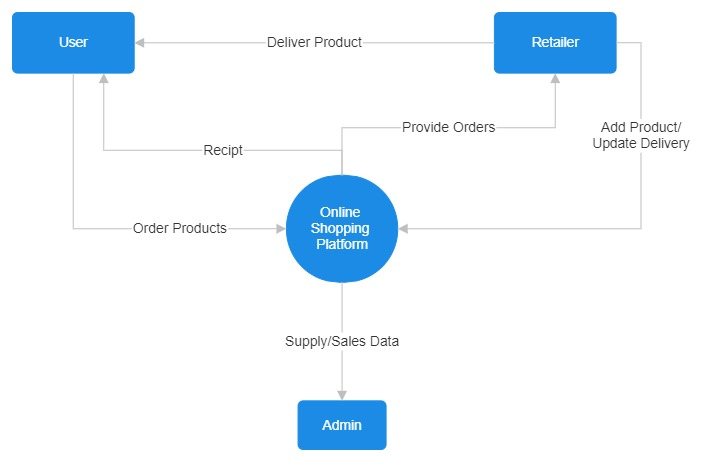
\includegraphics[width=0.8\textwidth]{cfd.jpg}
    \caption{Context Diagram for the E-commerce Platform}
\end{figure}


\section{Data Flow Diagrams (DFDs)}

\subsection{DFD-01: Money Flow and Operational Efficiency}
Designed to streamline payment gateway implementation and optimize administrative charges and retailer shares. Focuses on illustrating the flow of money, product deliveries, and user interactions within the platform.

\begin{figure}
    \centering
    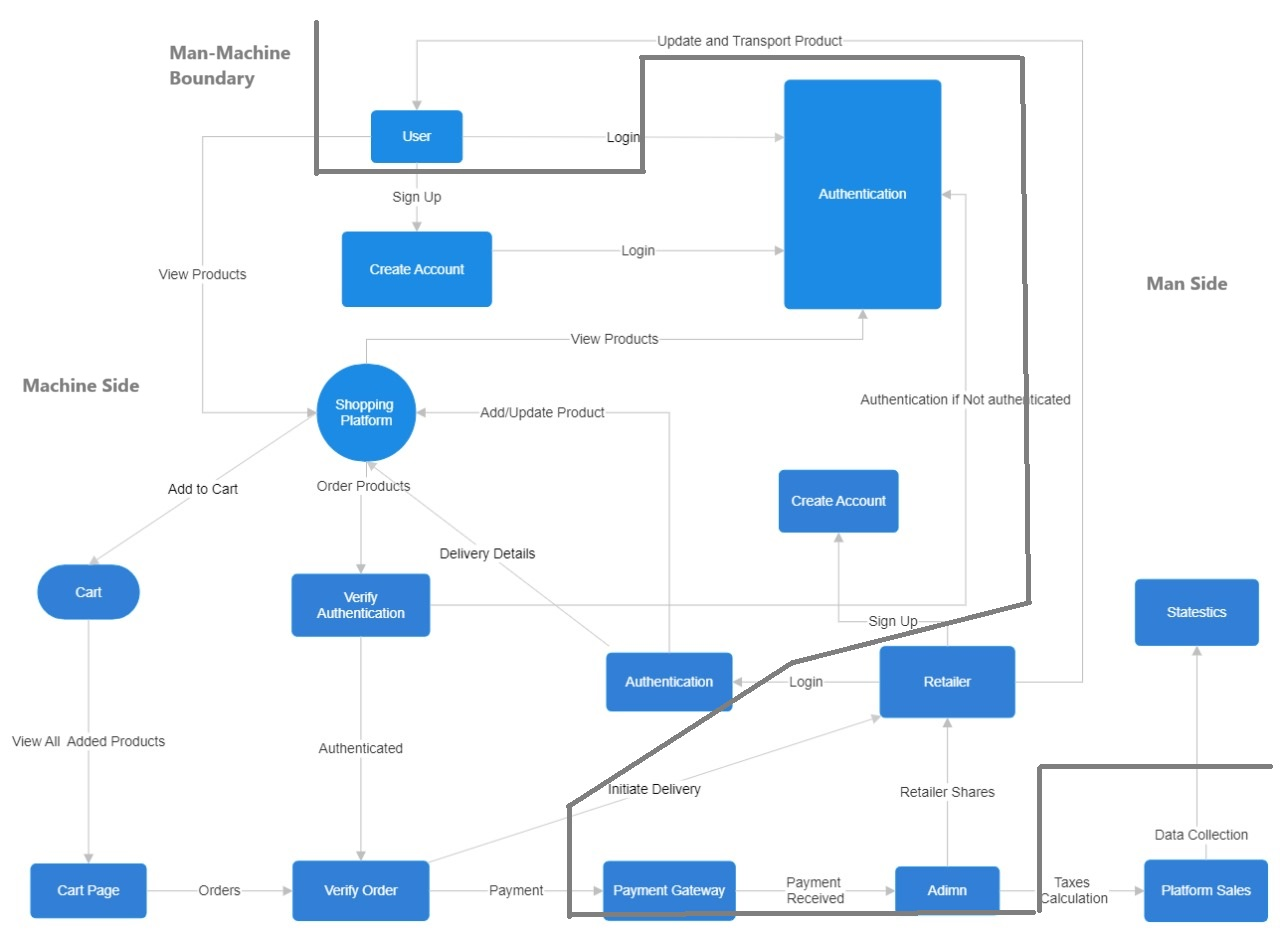
\includegraphics[width=0.8\textwidth]{dfd1.jpg}
    \caption{DFD-01: Money Flow and Operational Efficiency}
\end{figure}

\subsection{DFD-01 Workflow}

\begin{enumerate}

\item \textbf{User Registration and Product Viewing:}
   \begin{itemize}
      \item \textit{User Action:} A user can either sign up or log in to the e-commerce website.
      \item \textit{System Response:} Upon successful registration or login, the user gains access to their account, enabling them to view products on the shopping platform.
   \end{itemize}

\item \textbf{Cart Management:}
   \begin{itemize}
      \item \textit{User Action:} The user can add or update products in their shopping cart.
      \item \textit{System Response:} The shopping cart dynamically displays all added products, providing a convenient review mechanism for the user.
   \end{itemize}

\item \textbf{Order Placement and Verification:}
   \begin{itemize}
      \item \textit{User Action:} The user proceeds to order products from the cart.
      \item \textit{System Response:} Order processing involves authentication and payment verification to ensure a secure and valid transaction.
   \end{itemize}

\item \textbf{Payment Processing and Delivery Initiation:}
   \begin{itemize}
      \item \textit{User Action:} Payment is processed through a secure payment gateway.
      \item \textit{System Response:} Upon successful payment, the system initiates the delivery of ordered products, ensuring a smooth and efficient transaction.
   \end{itemize}

\item \textbf{Retailer Interaction and Product Updates:}
   \begin{itemize}
      \item \textit{Retailer Action:} Retailers can log in to the platform.
      \item \textit{System Response:} Retailers have the capability to share real-time updates on product availability and details, enriching the user experience.
   \end{itemize}

\item \textbf{Data Collection for Statistics:}
   \begin{itemize}
      \item \textit{Retailer Action:} Retailers contribute to data collection.
      \item \textit{System Response:} Data collected includes information on sales, product availability, and other relevant statistics crucial for platform management.
   \end{itemize}

\item \textbf{Sales and Taxes Calculation:}
   \begin{itemize}
      \item \textit{Retailer Action:} Retailers are actively involved in sales and taxes calculation.
      \item \textit{System Response:} The system leverages retailer-contributed data to calculate overall platform sales and taxes, providing valuable insights.
   \end{itemize}

\item \textbf{Administrative Oversight:}
   \begin{itemize}
      \item \textit{Admin Access:} The admin has privileged access to the system.
      \item \textit{System Response:} Admins can monitor and access comprehensive statistics, platform sales, and tax information, ensuring effective management and decision-making.
   \end{itemize}

\end{enumerate}


\subsection{DFD-02: Dual Payment Mode Emphasis}

Tailored to accommodate both regular users and retailers, emphasizing payment processes for both cash on delivery and online transactions. Prioritizes cart management, order initiation, and receipt generation for diverse payment methods.

\begin{figure}
    \centering
    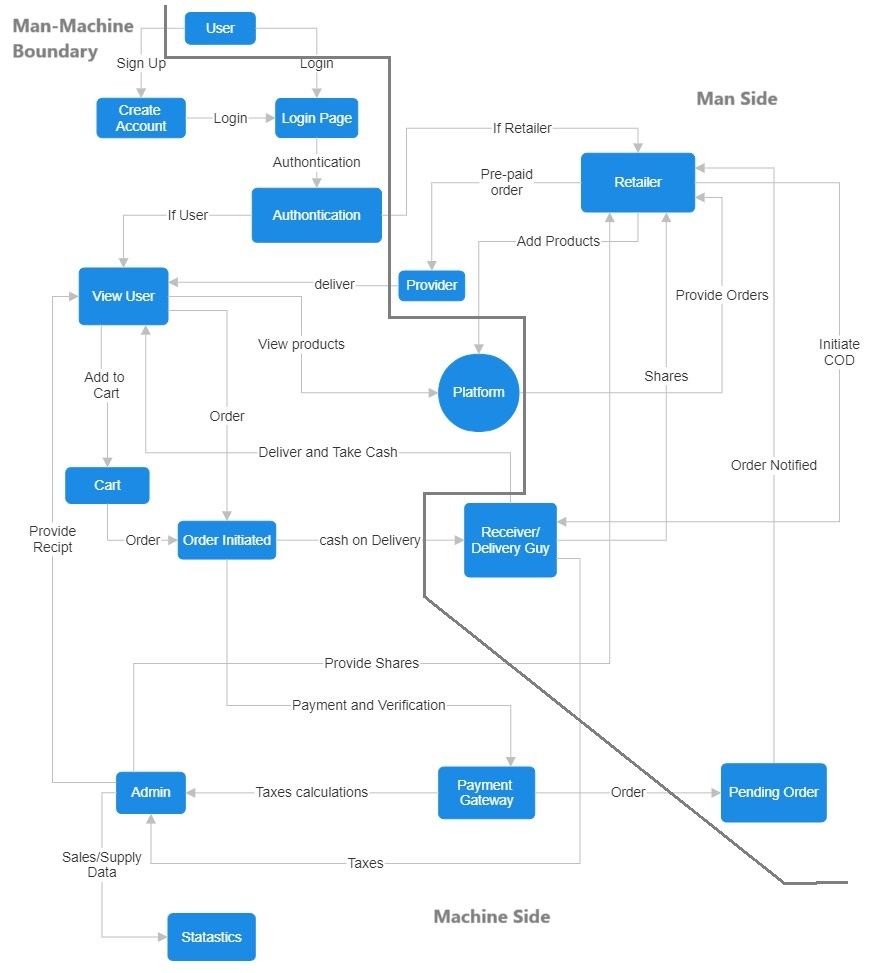
\includegraphics[width=0.8\textwidth]{dfd2.jpg}
    \caption{DFD-02: Dual Payment Mode Emphasis}
\end{figure}

\textbf{DFD-02 Workflow:}
\begin{enumerate}

\item \textbf{User Interaction for Regular Users and Retailers:}
   \begin{itemize}
      \item \textit{User Action:} Both regular users and retailers can interact with the platform.
      \item \textit{System Response:} The platform is designed to accommodate the needs of both user types, ensuring a seamless experience for all.
   \end{itemize}

\item \textbf{Payment Mode Selection:}
   \begin{itemize}
      \item \textit{User Action:} Users can choose between cash on delivery and online payment modes.
      \item \textit{System Response:} The system adapts to the selected payment mode, providing flexibility for diverse user preferences.
   \end{itemize}

\item \textbf{Cart Management:}
   \begin{itemize}
      \item \textit{User Action:} Users manage their shopping cart, adding, updating, or removing items.
      \item \textit{System Response:} Cart management remains a priority, ensuring a smooth and user-friendly experience for all transactions.
   \end{itemize}

\item \textbf{Order Initiation:}
   \begin{itemize}
      \item \textit{User Action:} Users initiate orders based on their cart contents.
      \item \textit{System Response:} The system processes order initiation, considering the selected payment mode and ensuring a secure transaction flow.
   \end{itemize}

\item \textbf{Receipt Generation:}
   \begin{itemize}
      \item \textit{User Action:} Upon order completion, users expect receipt generation.
      \item \textit{System Response:} Receipts are generated, providing users with comprehensive details of their transactions, regardless of the chosen payment mode.
   \end{itemize}

\end{enumerate}

\section{Justification for Choosing DFD-01}

After a thorough evaluation of various Data Flow Diagrams (DFDs), DFD-01 has been selected as the most suitable choice for the following compelling reasons:

\begin{enumerate}
  \item \textbf{User Differentiation:} DFD-01 effectively addresses the critical challenge of distinguishing between view users and retailers, mitigating ambiguity present in DFD-02. This distinction is pivotal for ensuring tailored interactions and personalized experiences for each user type, ultimately enhancing user satisfaction and platform usability.

  \item \textbf{Cash on Delivery Handling:} DFD-02 introduces unnecessary complexity in managing cash on delivery payments, impacting the clarity of the man-machine boundary. DFD-01, on the other hand, offers a straightforward approach to payment processing, minimizing potential confusion and ensuring a seamless transaction flow. This simplicity is crucial for a positive user experience, especially in handling diverse payment methods.

  \item \textbf{Reduced Man Side Complexity:} DFD-01 boasts a more streamlined man side within the man-machine boundary compared to DFD-02. The simplicity in the representation of user, retailer, and administrative interactions contributes to enhanced operational clarity. This clarity facilitates easier system understanding, maintenance, and future scalability.

  \item \textbf{Enhanced Security Measures:} DFD-01 prioritizes security by clearly outlining the authentication and payment verification processes. This meticulous attention to security ensures that transactions are secure and valid, instilling trust in users and promoting the platform's credibility.

  \item \textbf{Optimized User Experience:} DFD-01 is designed to optimize the overall user experience by focusing on essential functionalities such as order placement, payment processing, and product delivery. The streamlined workflow ensures that users can navigate the platform effortlessly, leading to increased user satisfaction and engagement.

  \item \textbf{Scalability and Future Development:} DFD-01 lays a foundation for scalability and future development. Its clear representation of user roles and interactions allows for easier integration of additional features, such as new payment gateways or expanded product management capabilities. This scalability is essential for adapting to evolving user needs and market trends.

  \item \textbf{Consistent Data Flow:} DFD-01 ensures a consistent and logical flow of data throughout the system. This consistency is crucial for maintaining data integrity and avoiding potential errors or discrepancies in transaction processing.

\end{enumerate}

\section{Function Point Analysis}

\subsection{External Inputs (EI)}
\begin{itemize}
    \item \textbf{Simple:} Authentication (User/Customer), Login (User/Customer), SignUp (User/Customer), Authentication (Admin), Login (Admin), SignUp (Admin), Authentication (Retailers)
    \item \textbf{Average:} Profile (User/Customer), Product Management (Admin), Edit profile (Retailers), View Cart Contents (Cart), Remove Items from Cart (Cart), Add Items to Cart (Cart), View Order History (Order Management), Generate Invoices (Order Management), Search for Products within the platform
\end{itemize}
\textbf{Total External Inputs (EI):} 19

\subsection{External Outputs (EO)}
\begin{itemize}
    \item \textbf{Simple:} None
    \item \textbf{Average:} View/Edit Profile Information (User/Customer), Add, Edit, Delete Product Listings (Admin), Edit profile (Retailers), View Cart Contents (Cart), View Order History (Order Management), Generate Invoices (Order Management)
\end{itemize}
\textbf{Total External Outputs (EO):} 6

\subsection{Logical Internal Files (ILF)}
\begin{itemize}
    \item \textbf{Simple:} None
    \item \textbf{Average:} Profile Information (User/Customer), Product Listings (Admin), Retailer Profile Information (Retailers), Cart Contents (Cart), Order History (Order Management), Invoices (Order Management)
\end{itemize}
\textbf{Total Logical Internal Files (ILF):} 6

\subsection{External Interface Files (EIF)}
\begin{itemize}
\item Node
\end{itemize}

\subsection{External Inquiries (EQ)}
\begin{itemize}
\item Node
\end{itemize}
\subsection{Function Point Contribution Table}
\begin{center}
\begin{tabular}{|c|c|c|c|}
\hline
Function Type & Simple & Average & Complex \\
\hline
External Input & 3 & 4 & 7 \\
External Output & 4 & 5 & 10 \\
Logical Internal File & 7 & 10 & 15 \\
\hline
\end{tabular}
\end{center}

\subsection{Classifying Elements and Calculating Unadjusted Function Points (UFP)}
\begin{itemize}
    \item \textit{Classifying Elements:} Follow the classification based on complexity.
    \item \textit{Calculating UFP:} Use the weighted sum formula.
\end{itemize}

\textbf{Result:}

\textit{Unadjusted Function Points (UFP):} 99

\end{document}
